\chapter{Additional Figures}

\begin{figure}
    \centering
    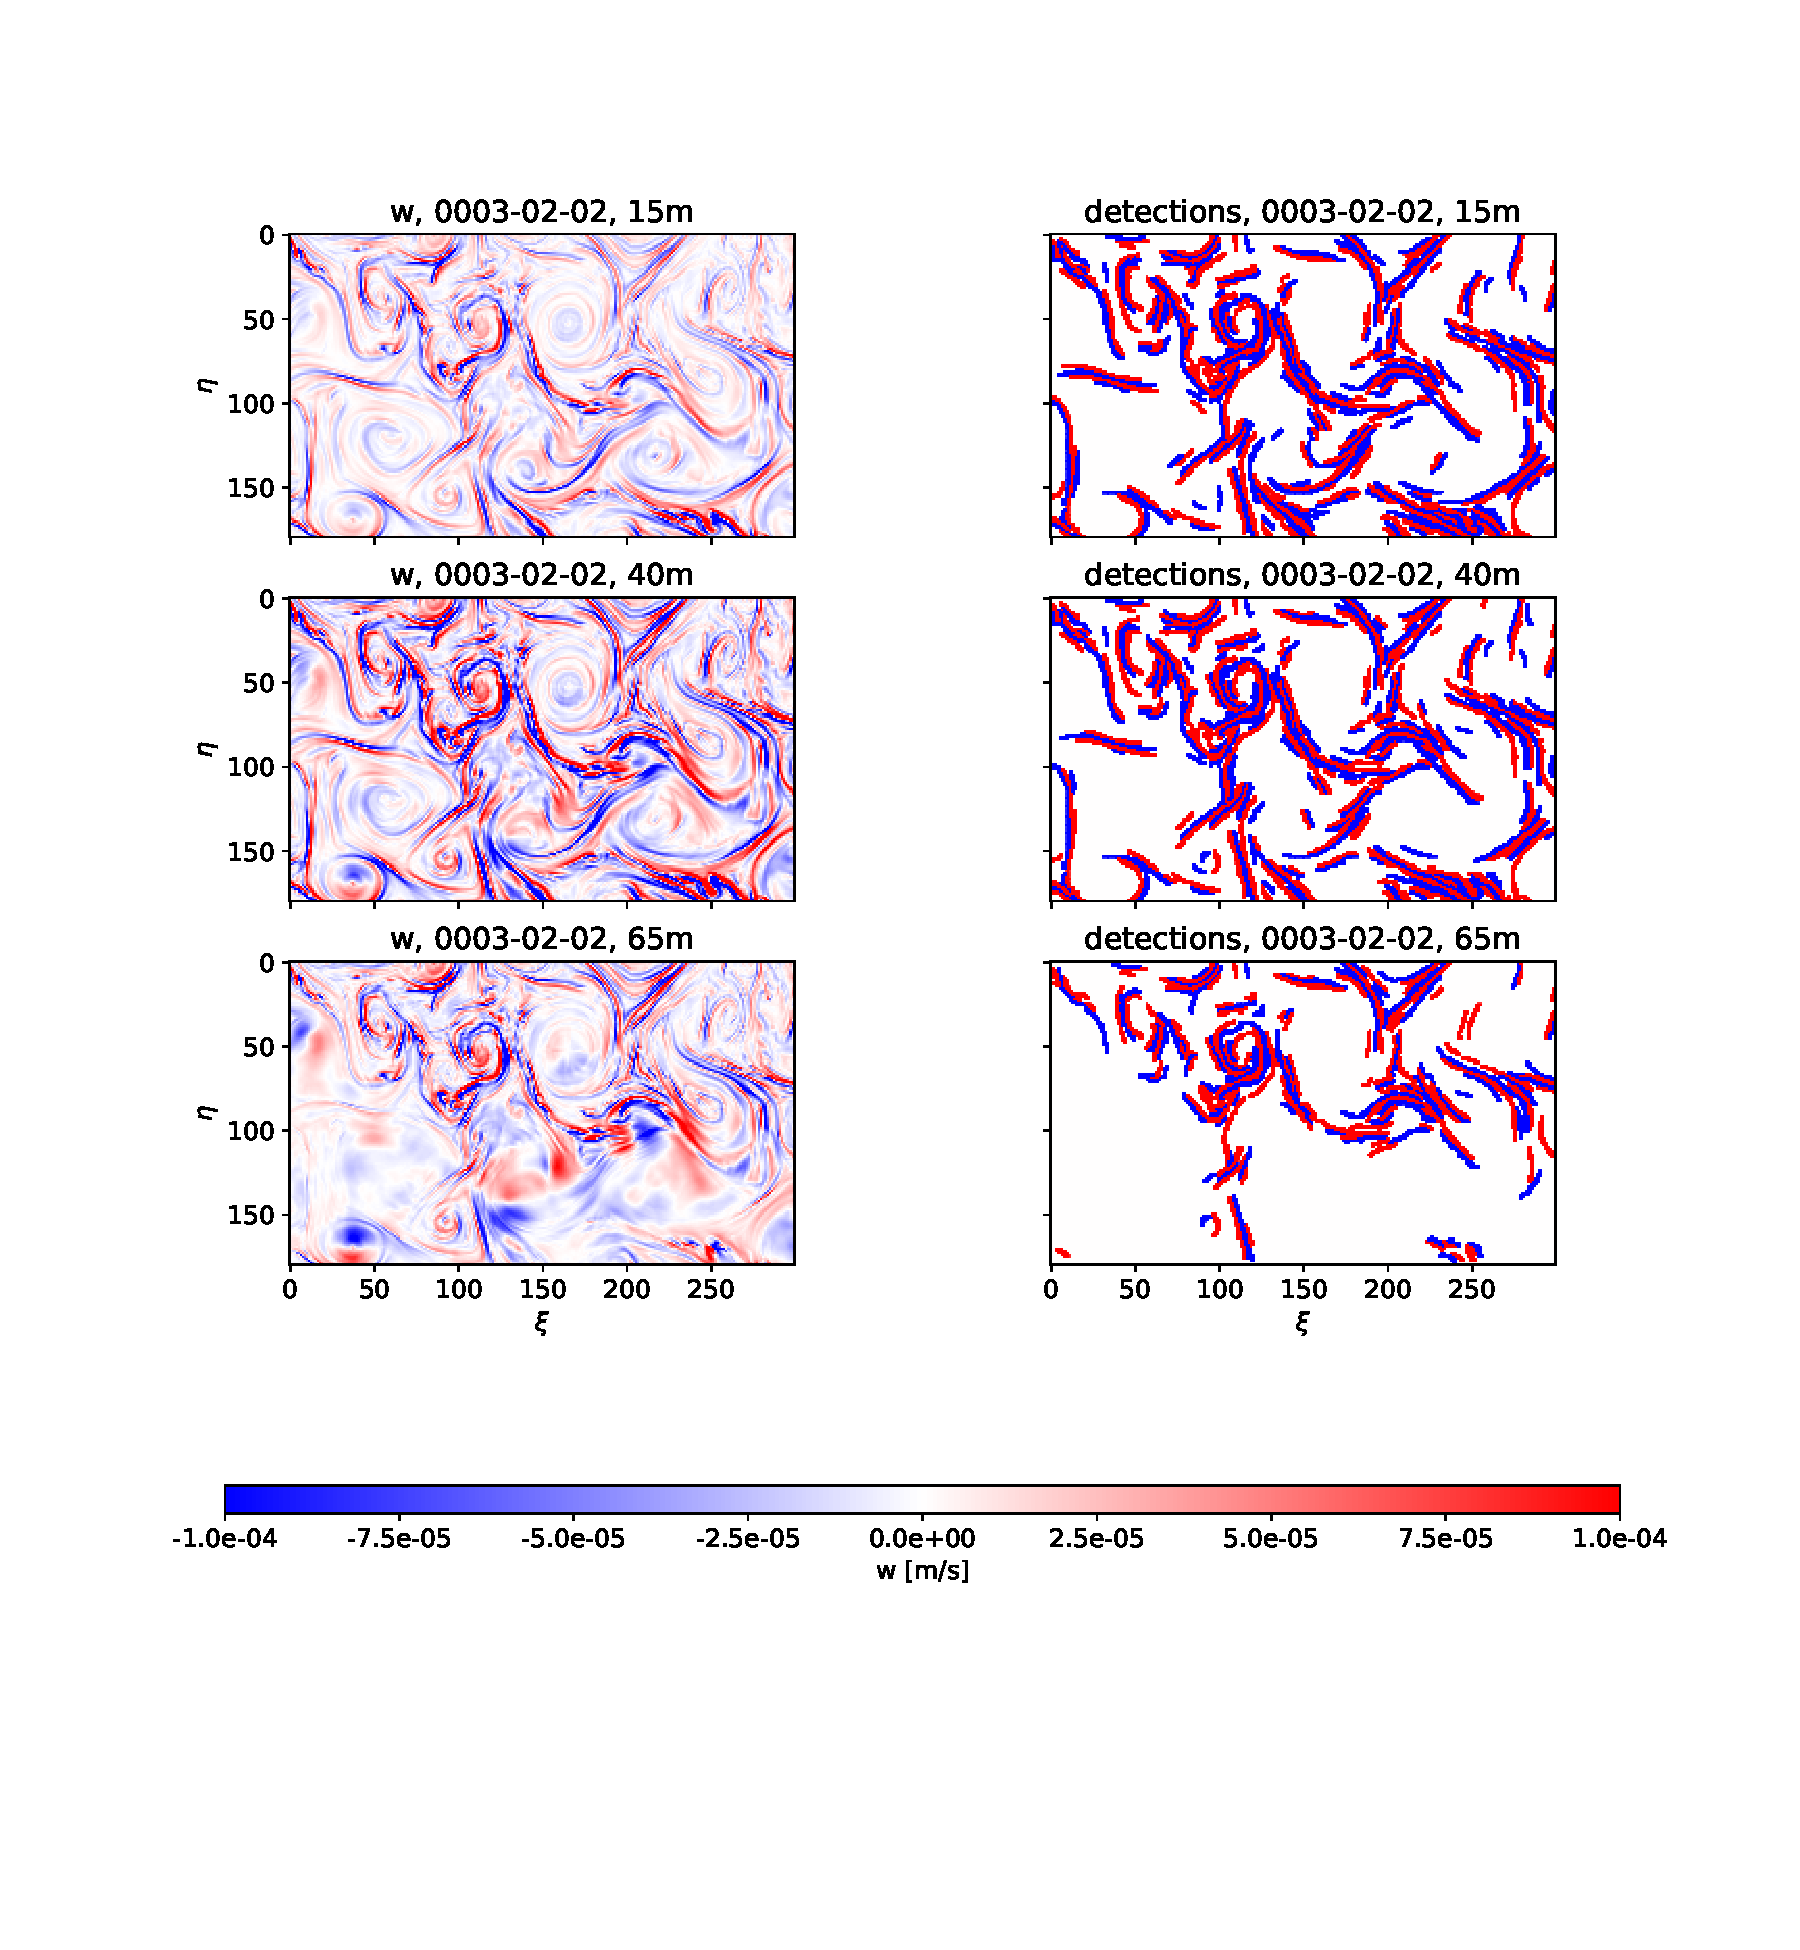
\includegraphics[width=16cm, trim=2.5cm 0 0 2cm]{figures/eval_det_subm_winter.pdf}
    \caption[Detection results for HR in winter: I]{\textbf{Detection results for HR in winter: I}. Data from 0003-02-02 is shown for different depths. The vertical velocity is shown left, the detection results right.}\label{fig:subm_det_winter}
\end{figure}

\begin{figure}
    \centering
    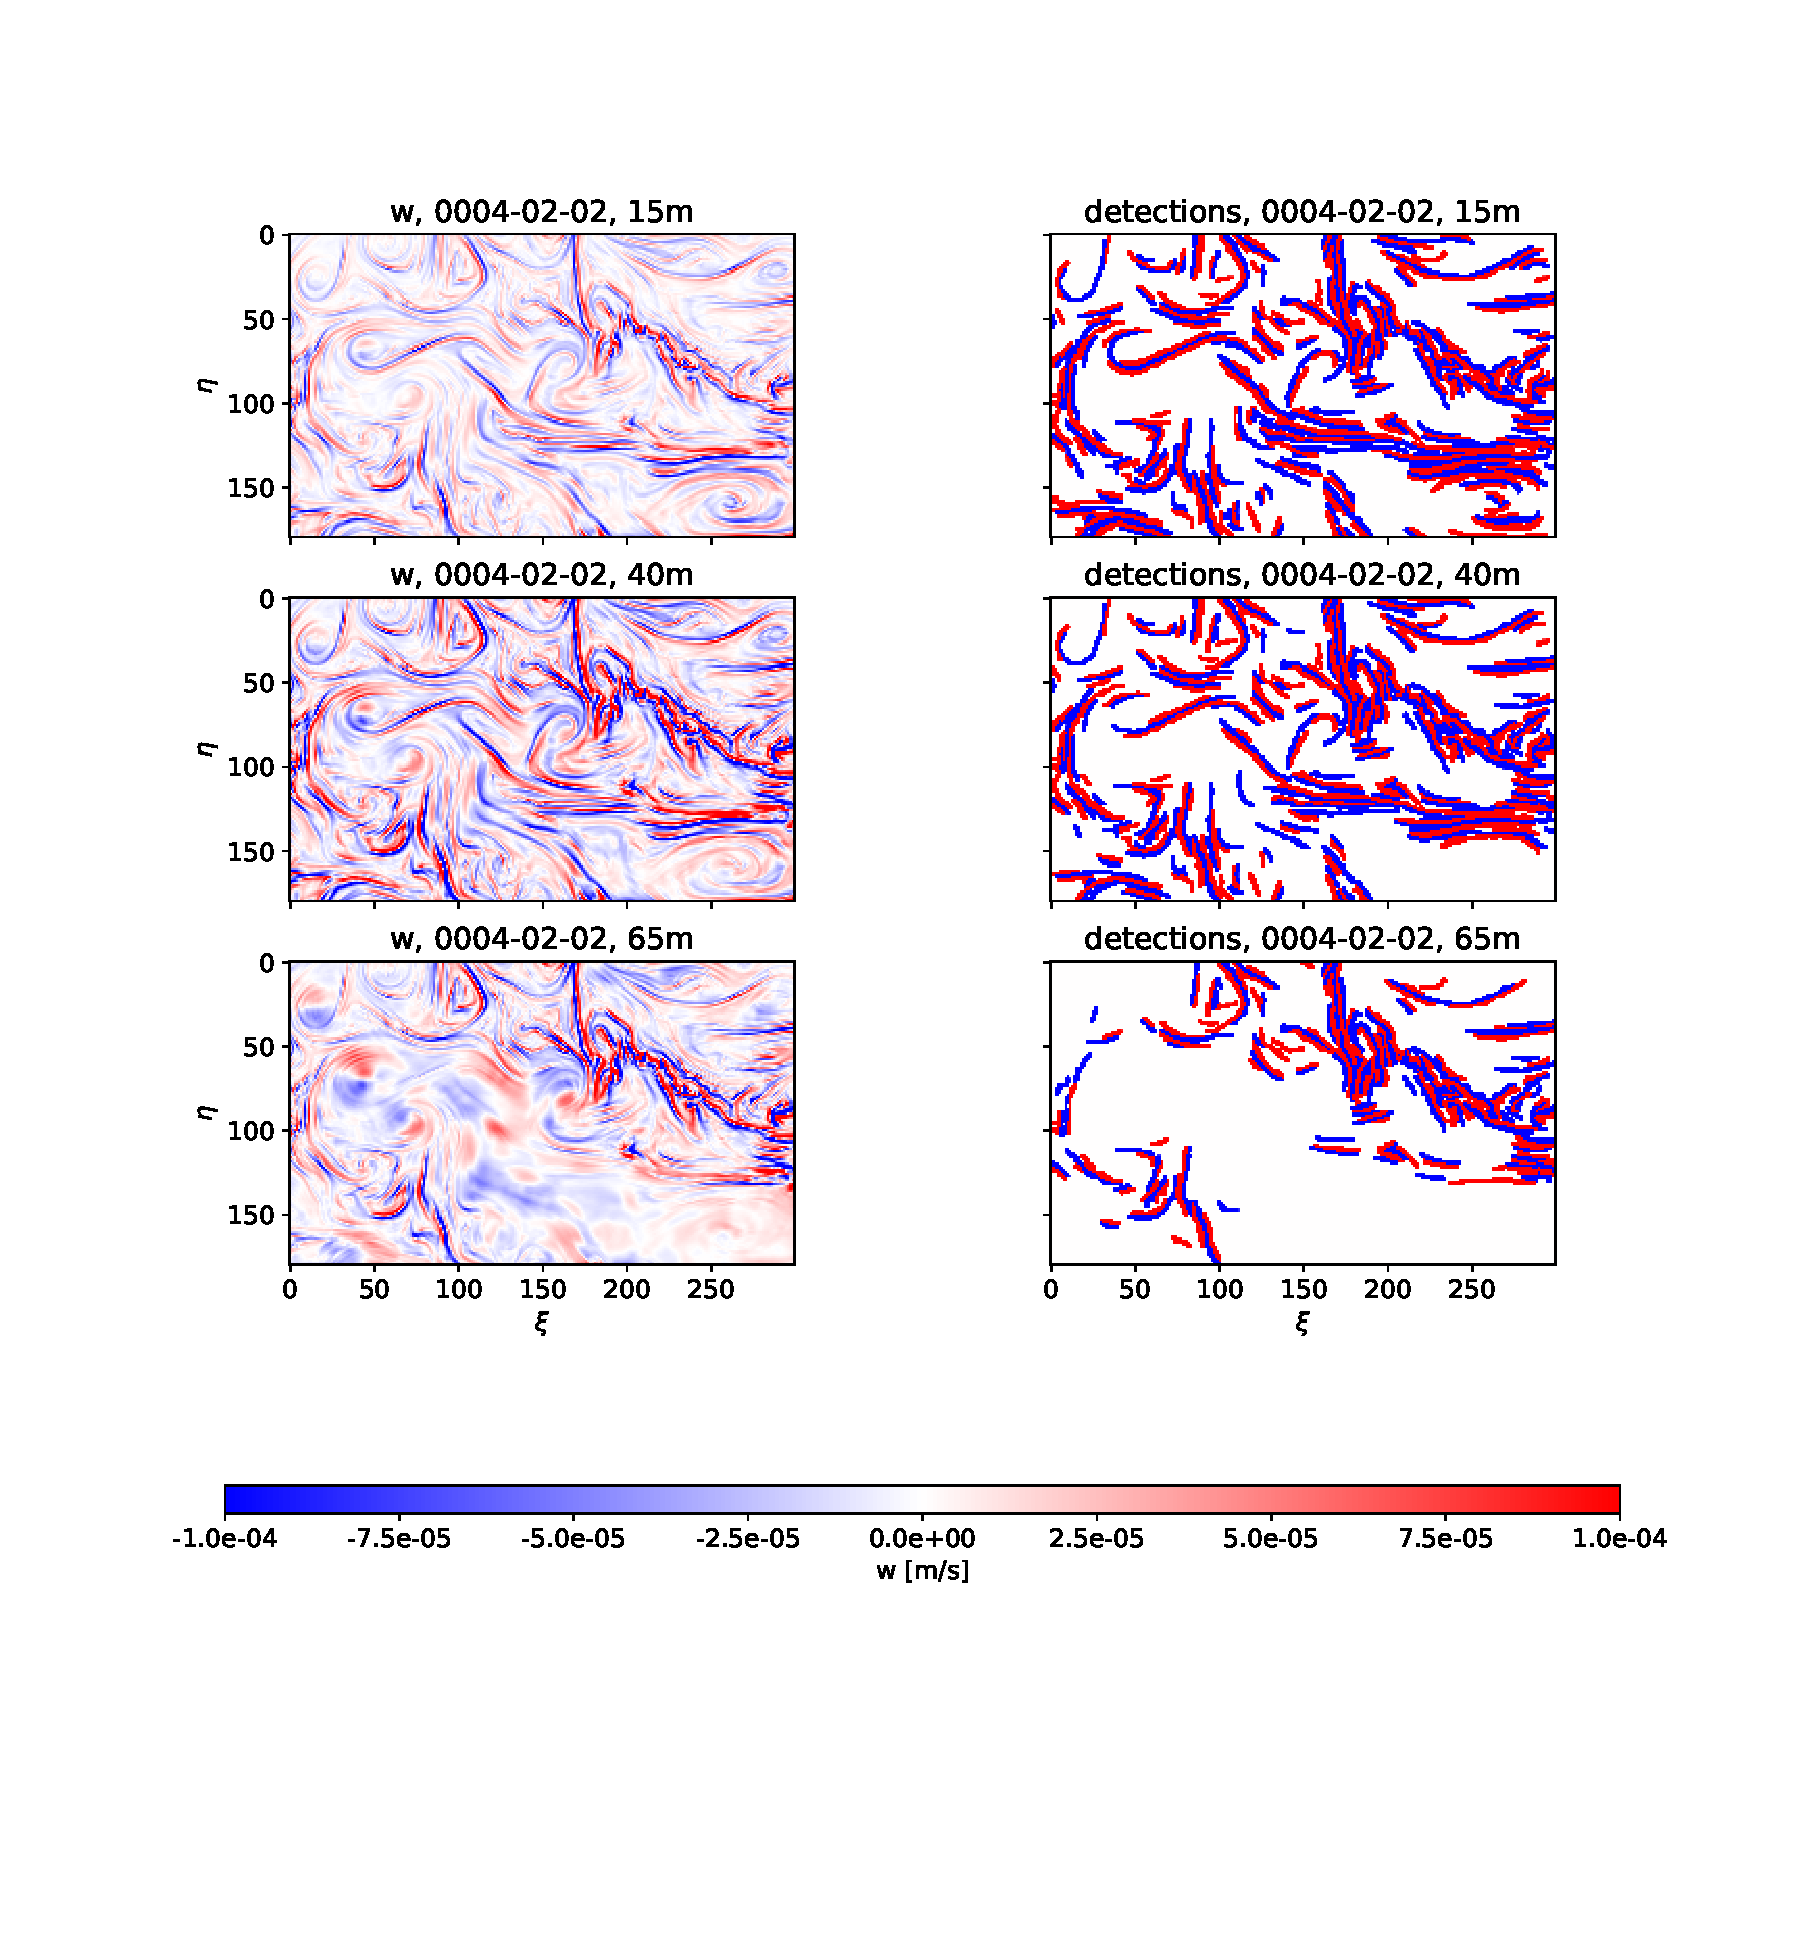
\includegraphics[width=16cm, trim=2.5cm 0 0 2cm]{figures/eval_det_subm_winter2.pdf}
    \caption[Detection results for HR in winter: II]{\textbf{Detection results for HR in winter: II}. Data from 0004-02-02 is shown for different depths. The vertical velocity is shown left, the detection results right.}\label{fig:subm_det_winter2}
\end{figure}

\begin{figure}
    \centering
    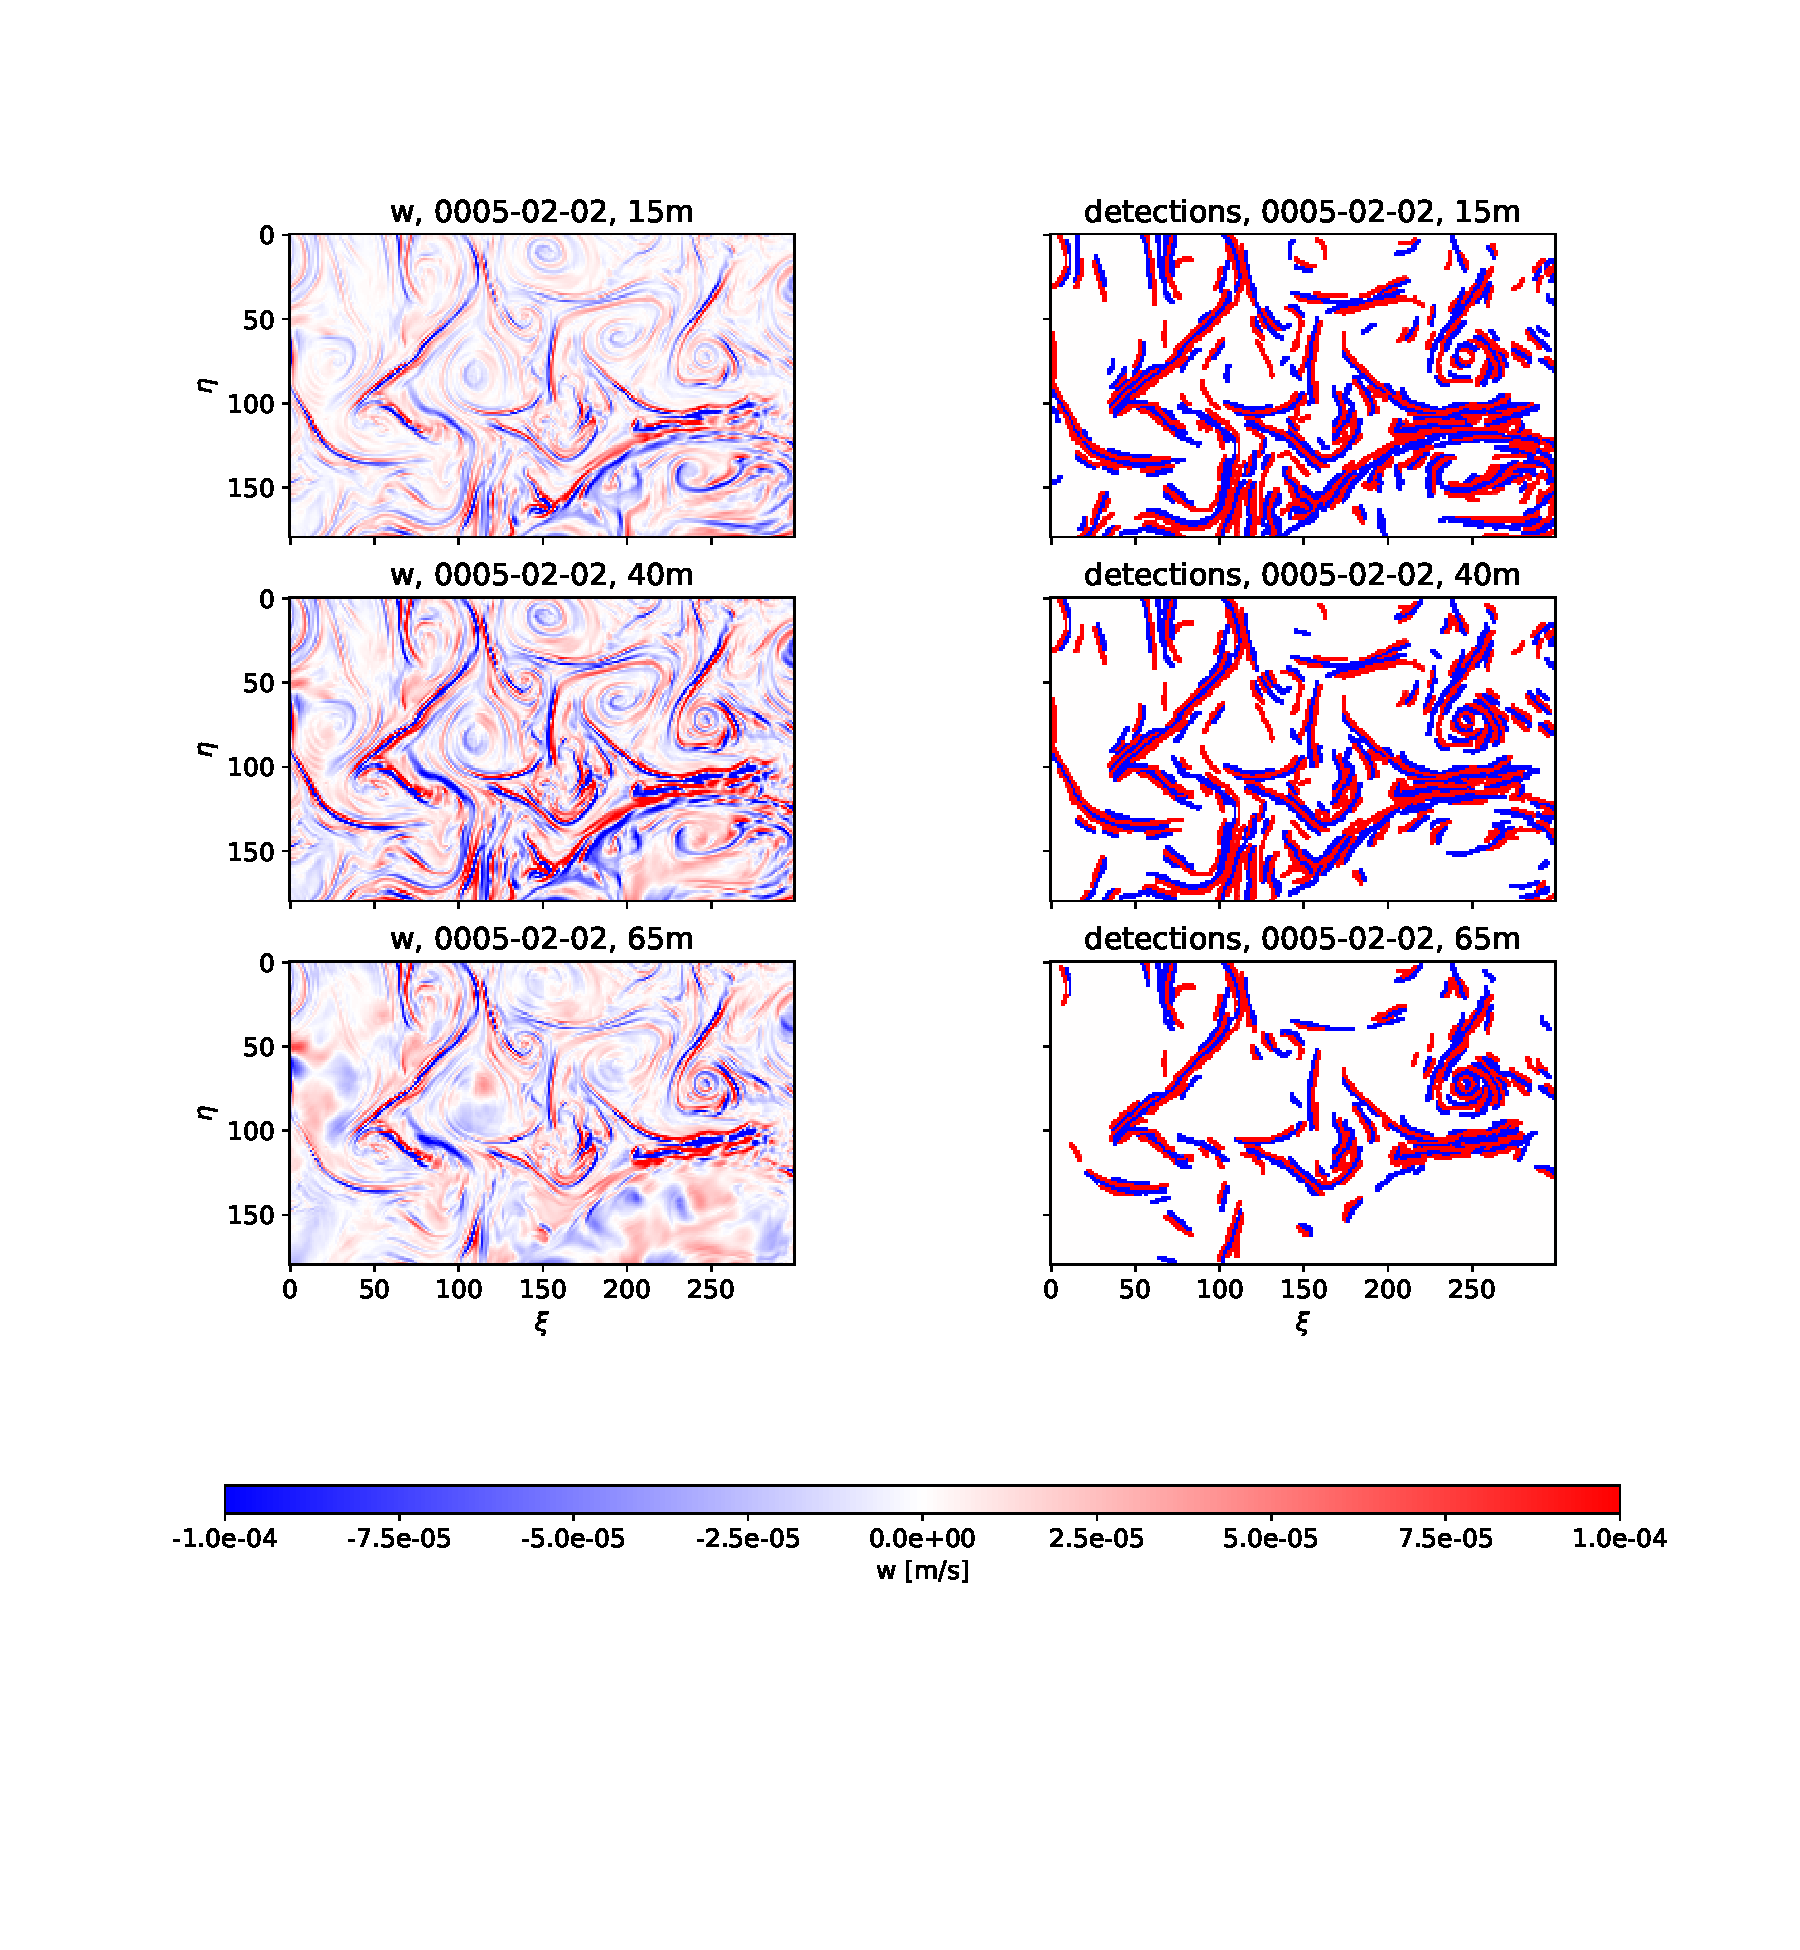
\includegraphics[width=16cm, trim=2.5cm 0 0 2cm]{figures/eval_det_subm_winter3.pdf}
    \caption[Detection results for HR in winter: III]{\textbf{Detection results for HR in winter: III}. Data from 0005-02-02 is shown for different depths. The vertical velocity is shown left, the detection results right.}\label{fig:subm_det_winter3}
\end{figure}

\begin{figure}
    \centering
    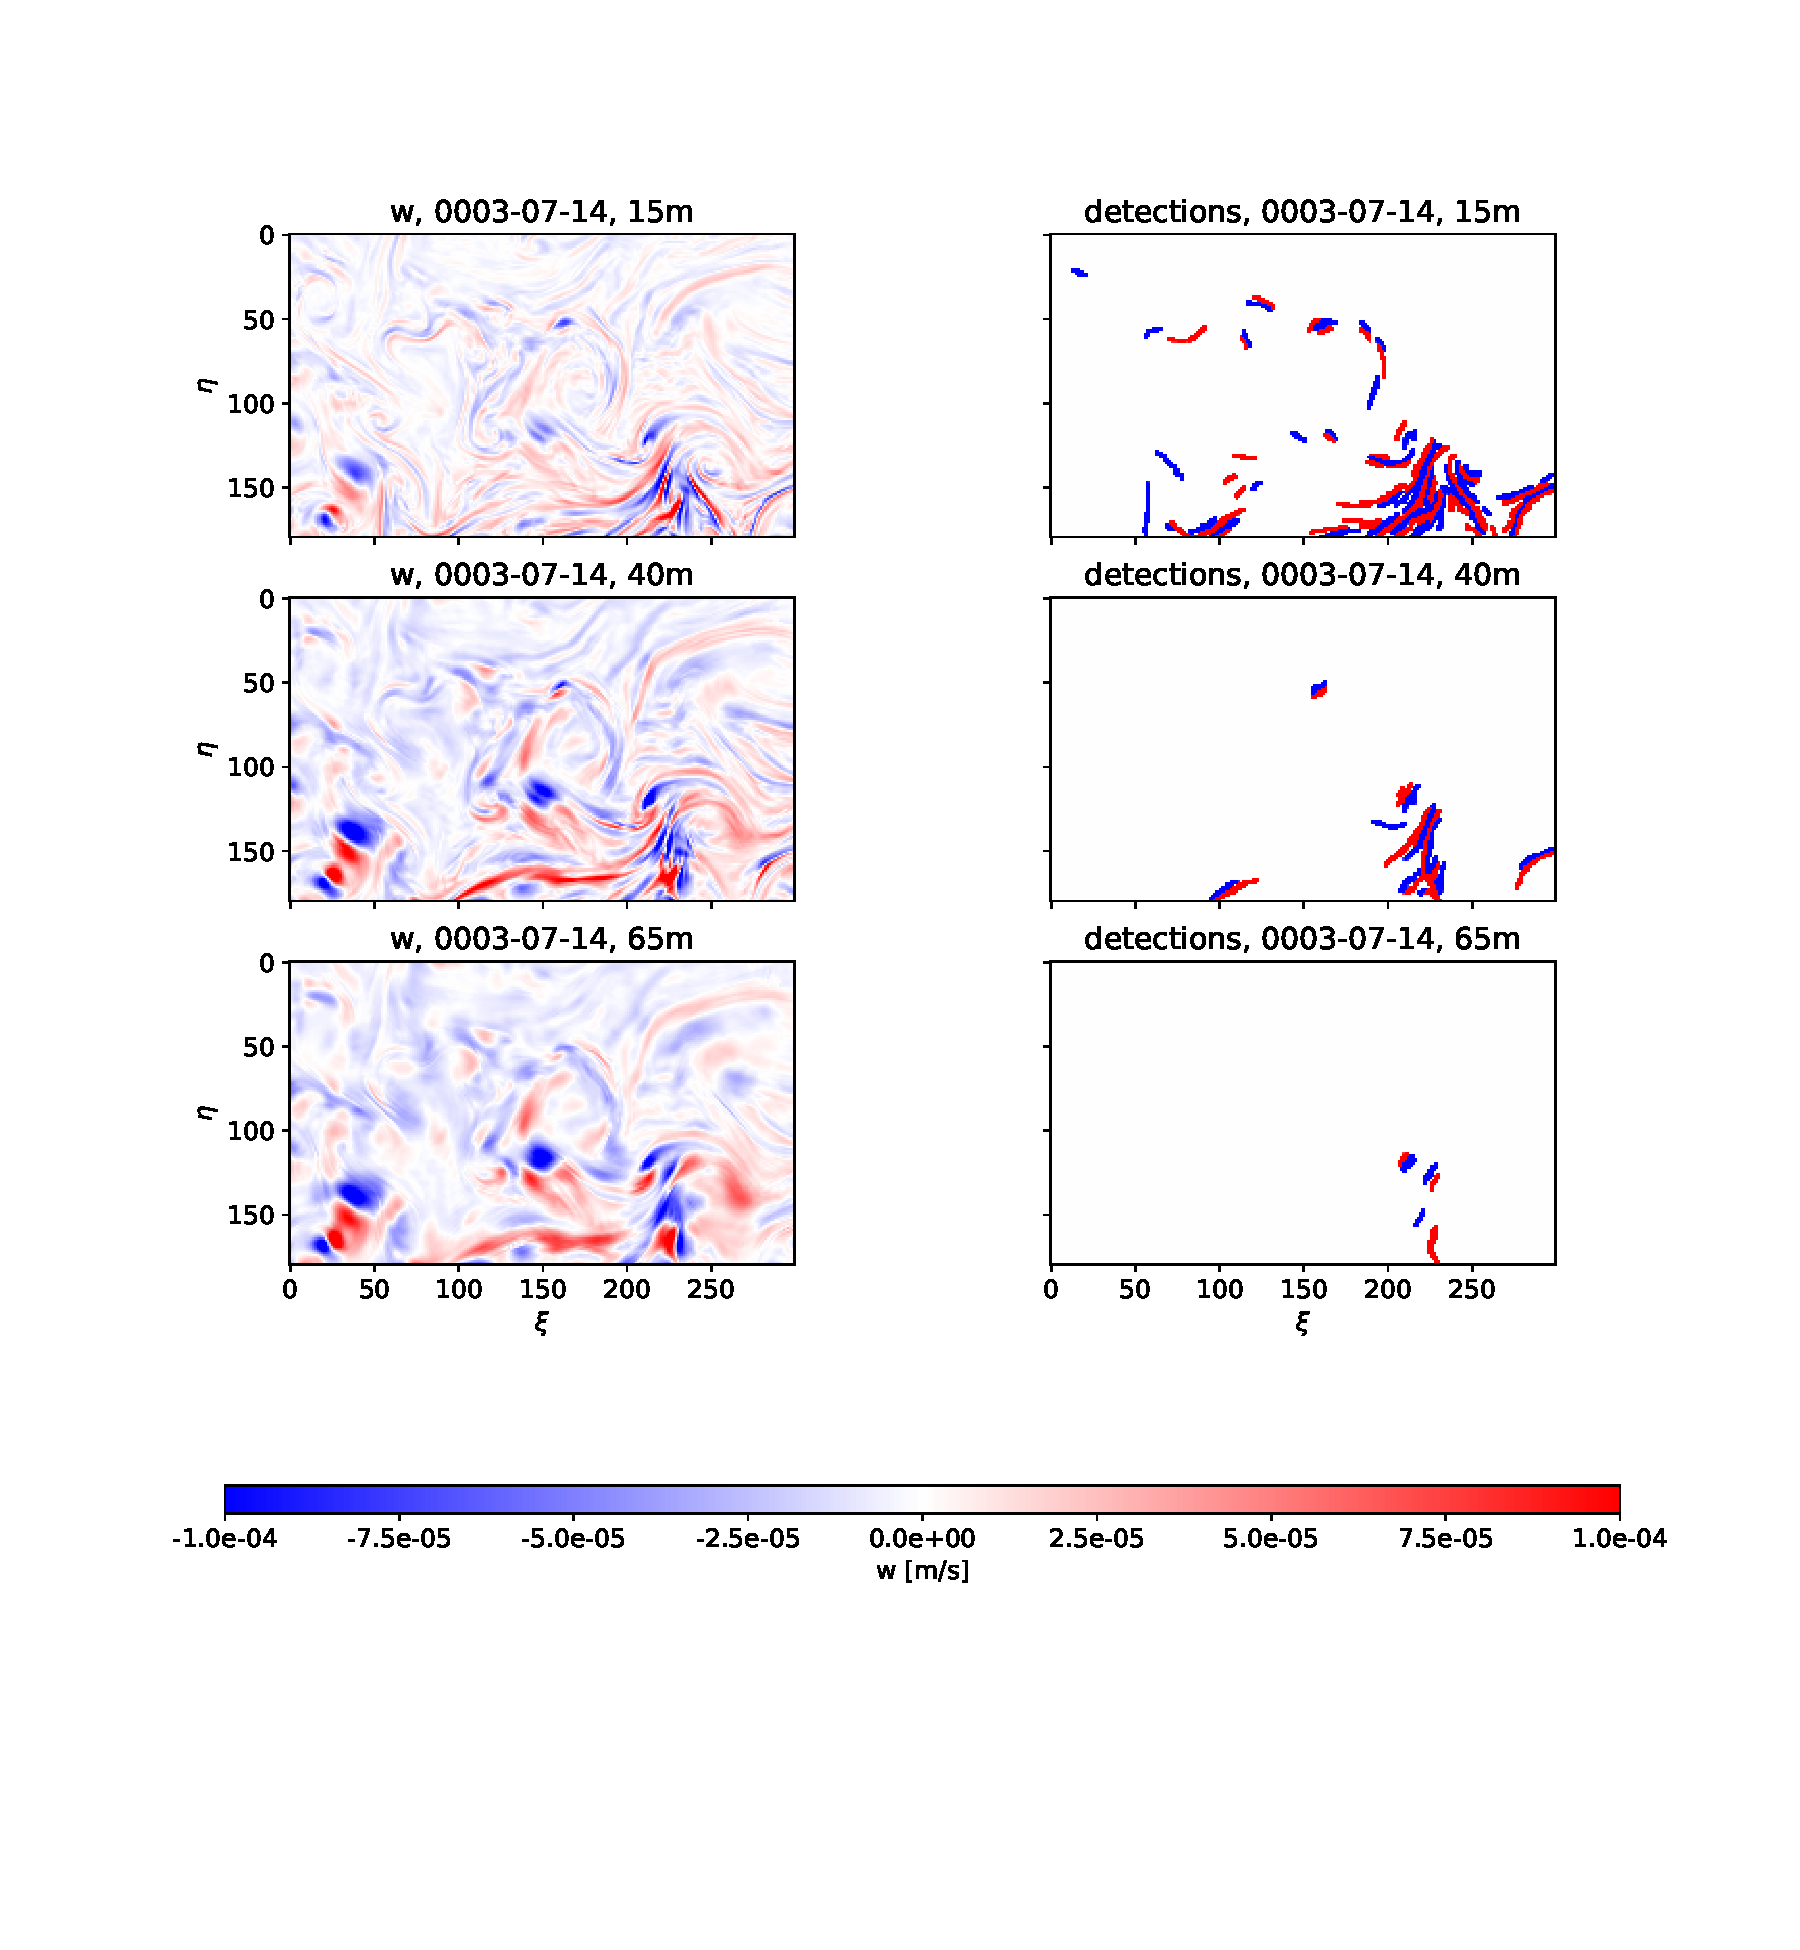
\includegraphics[width=16cm, trim=2.5cm 0 0 2cm]{figures/eval_det_subm_summer.pdf}
    \caption[Detection results for HR in summer]{\textbf{Detection results for HR in summer}. Data from 0003-07-14 is shown for different depths. The vertical velocity is shown left, the detection results right.}\label{fig:subm_det_summer}
\end{figure}

\begin{figure}
    \centering
    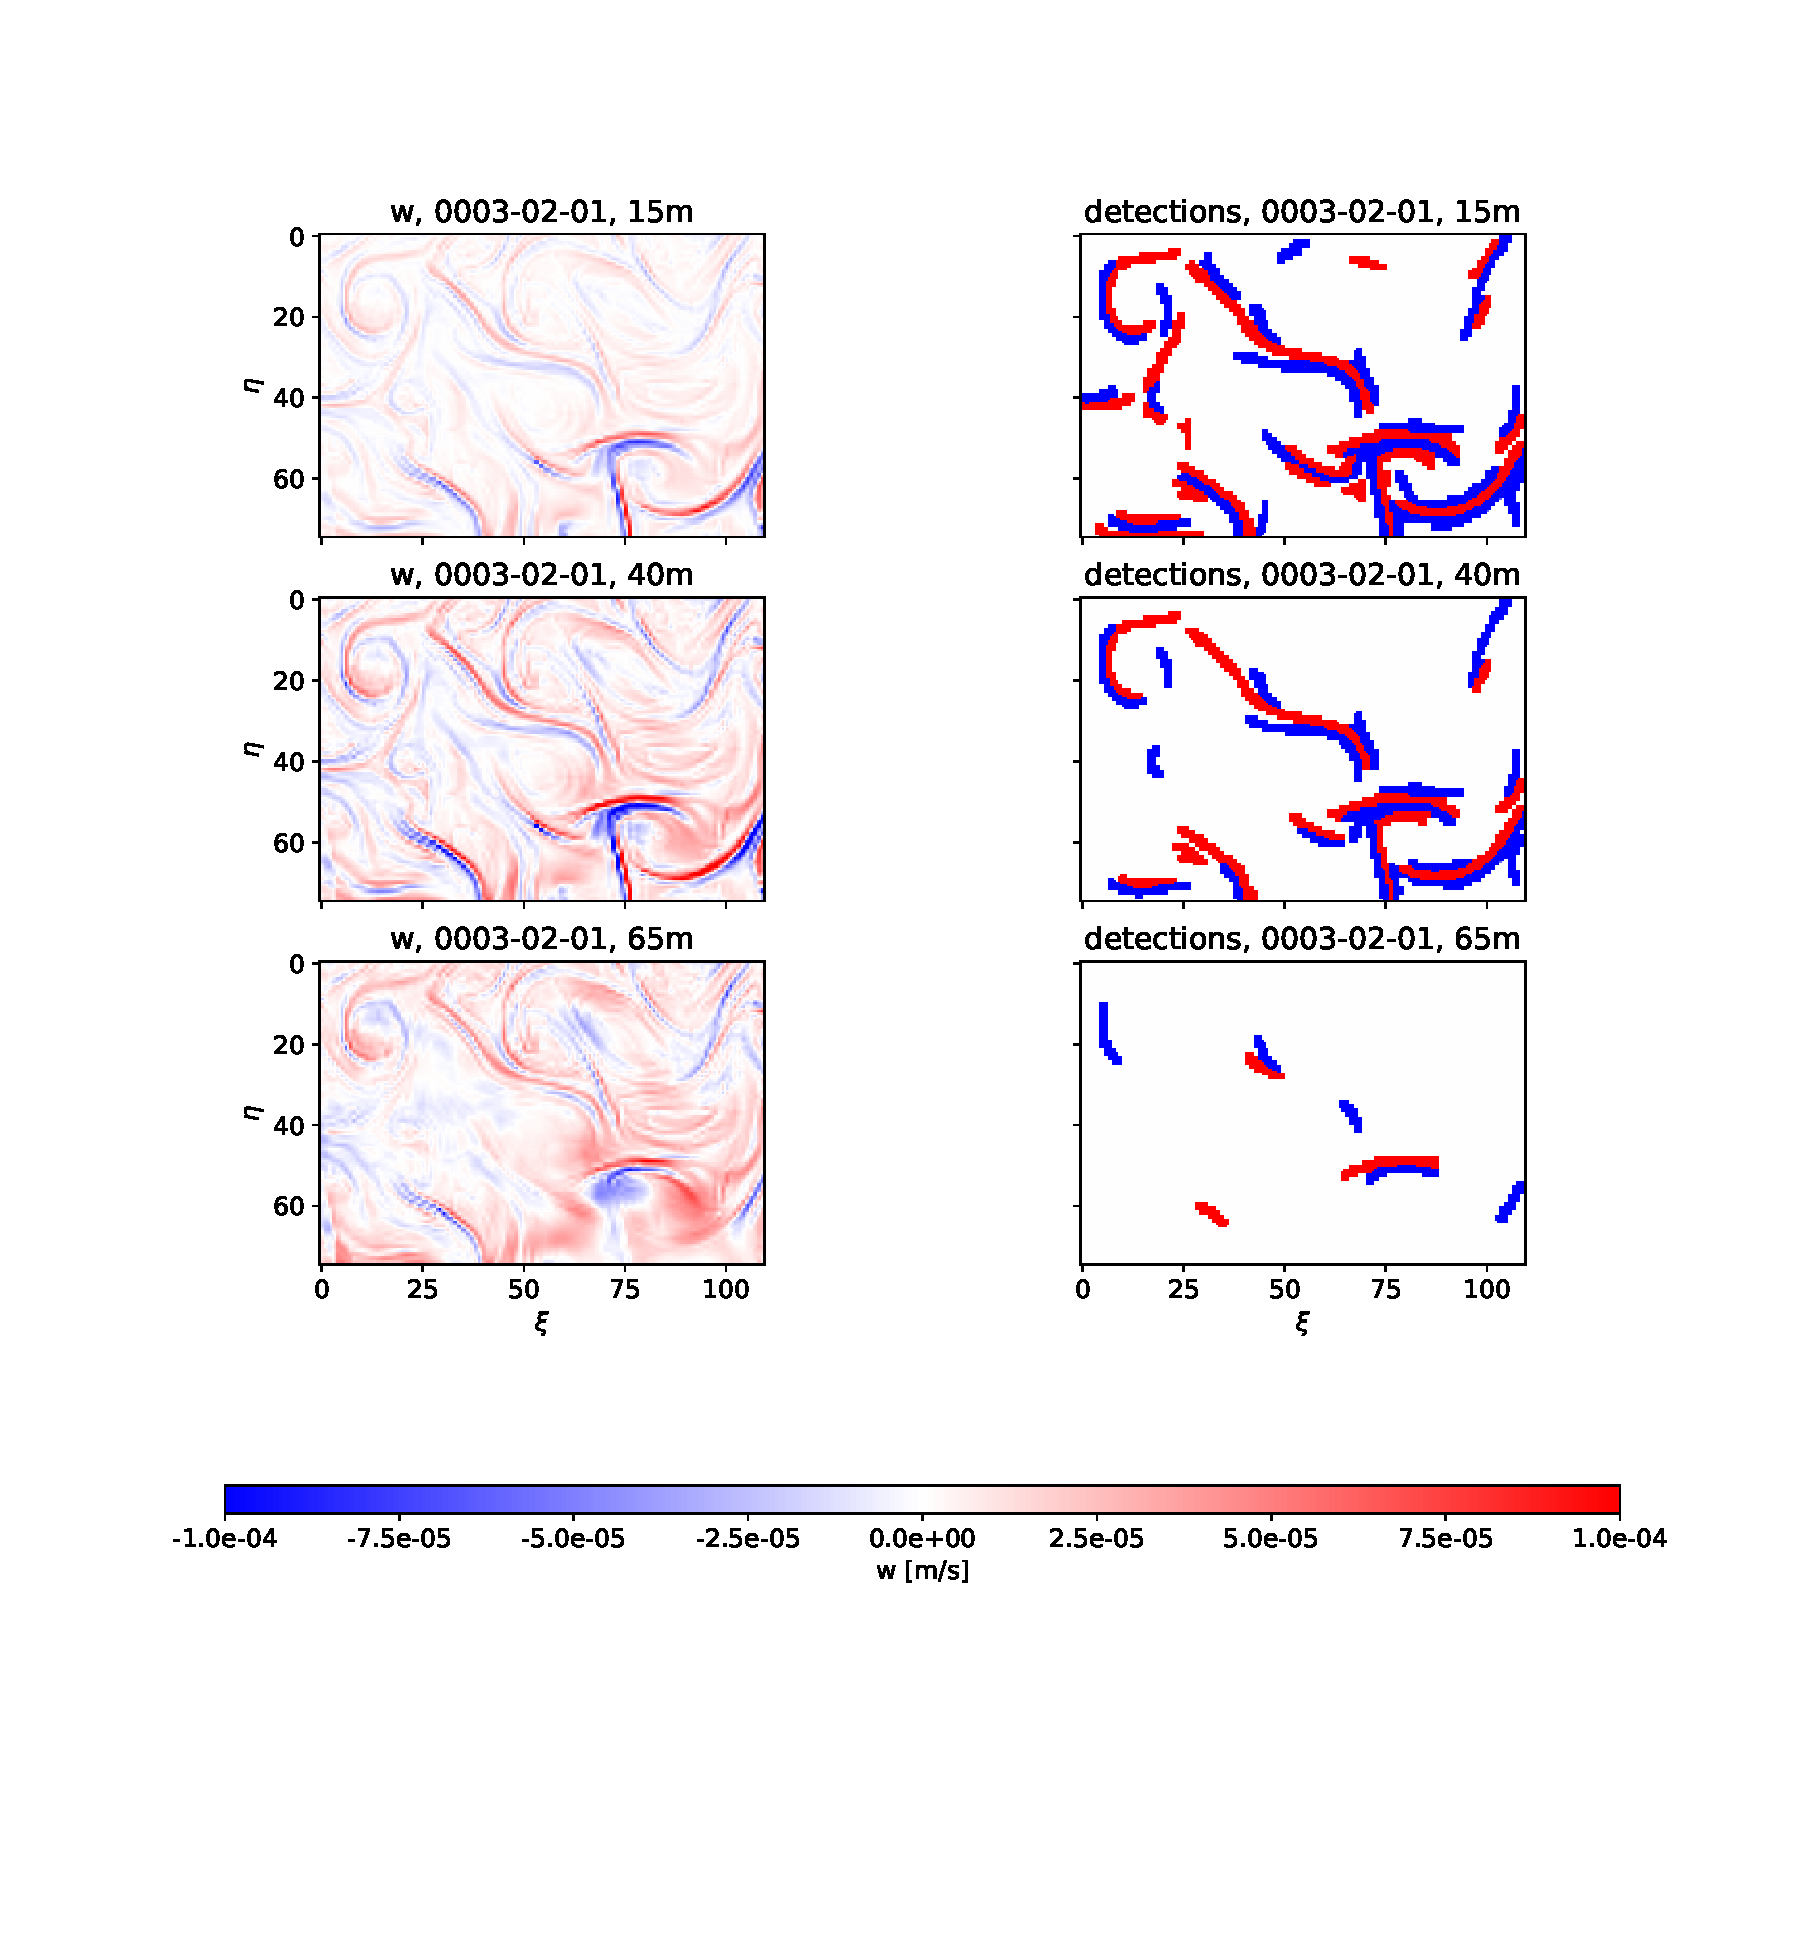
\includegraphics[width=16cm, trim=2.5cm 0 0 2cm]{figures/eval_det_meso_winter.pdf}
    \caption[Detection results for LR in winter: I]{\textbf{Detection results for LR in winter: I}. Data from 0003-02-01 is shown for different depths. The vertical velocity is shown left, the detection results right.}\label{fig:subm_det_winter_meso}
\end{figure}

\begin{figure}
    \centering
    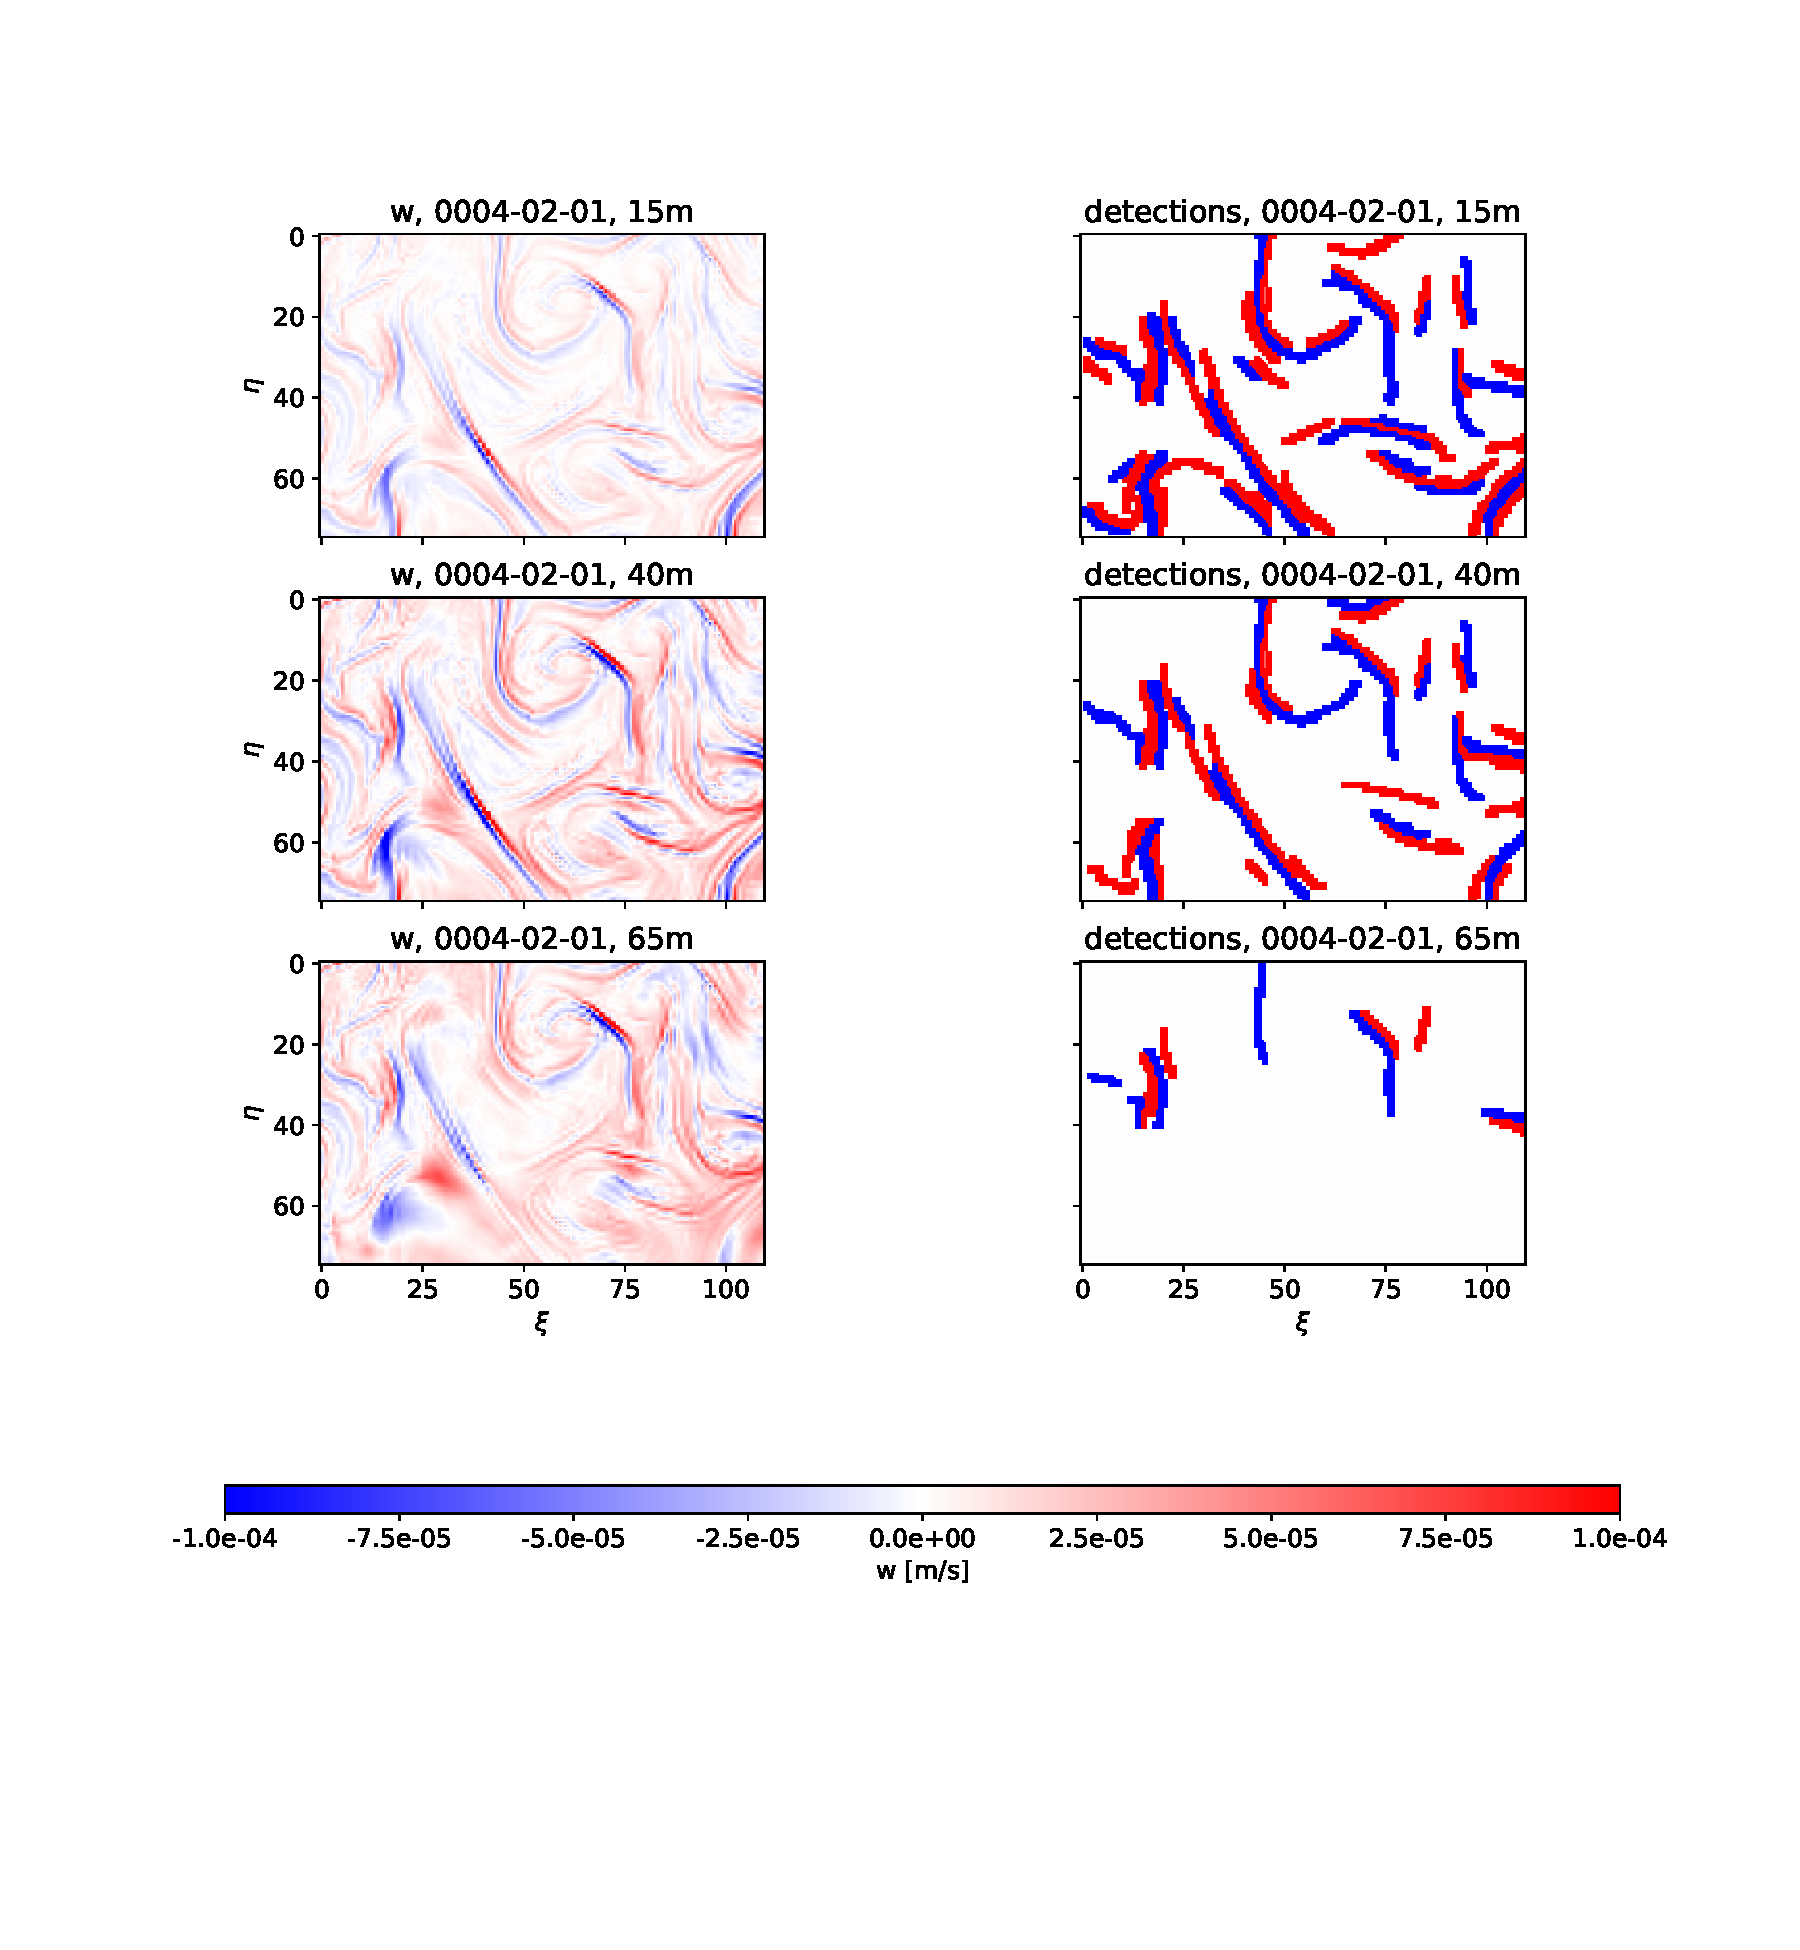
\includegraphics[width=16cm, trim=2.5cm 0 0 2cm]{figures/eval_det_meso_winter2.pdf}
    \caption[Detection results for LR in winter: II]{\textbf{Detection results for LR in winter: II}. Data from 0004-02-01 is shown for different depths. The vertical velocity is shown left, the detection results right.}\label{fig:subm_det_winter_meso2}
\end{figure}

\begin{figure}
    \centering
    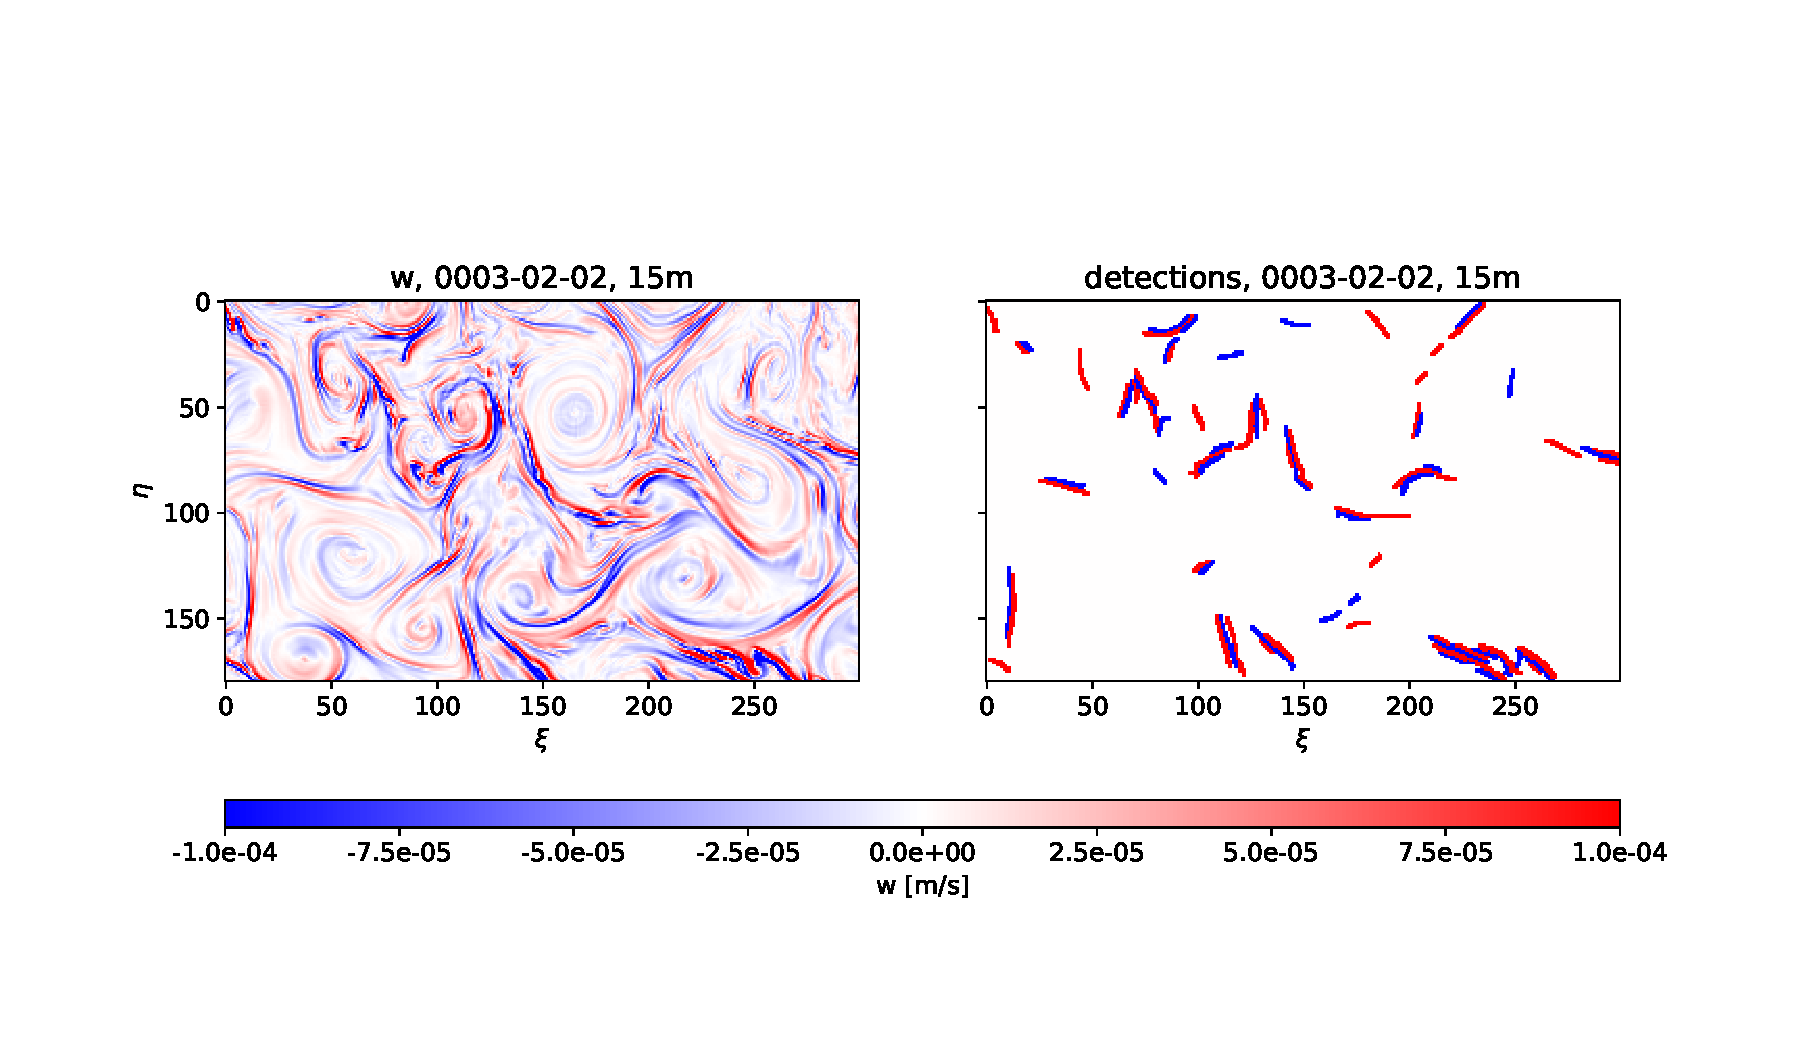
\includegraphics[width=16cm, trim=2.5cm 0 0 2cm]{figures/eval_det_sig_sm.pdf}
    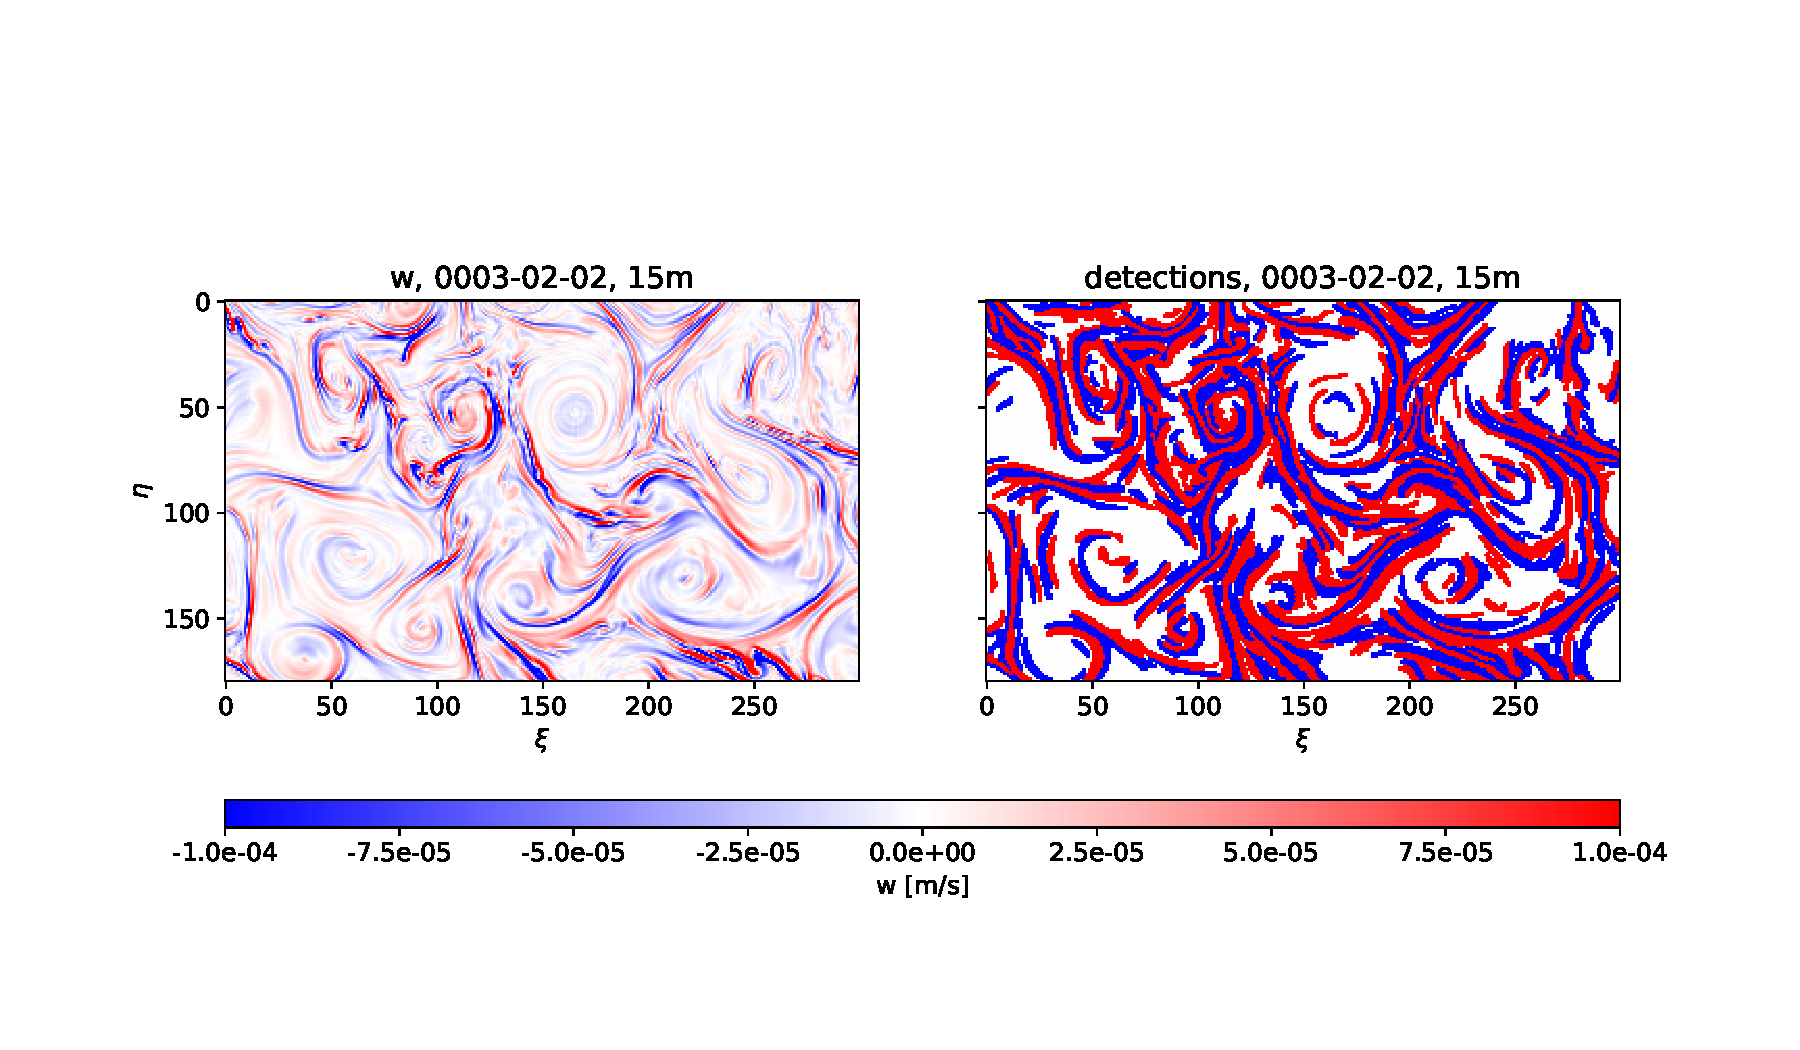
\includegraphics[width=16cm, trim=2.5cm 0 0 2cm]{figures/eval_det_sig_lg.pdf}
    \caption[Detection results for different $\sigma_\text{lat}$]{\textbf{Detection results for different $\sigma_\text{lat}$}. Data from 0003-02-01 is shown for $\sigma_\text{lat} = 1$ (top) and $\sigma_\text{lat} = 4$ (bottom). See \autoref{fig:subm_det_winter} for $\sigma_text{lat} = 2$.}\label{fig:subm_det_sigma}
\end{figure}

\begin{figure}
    \centering
    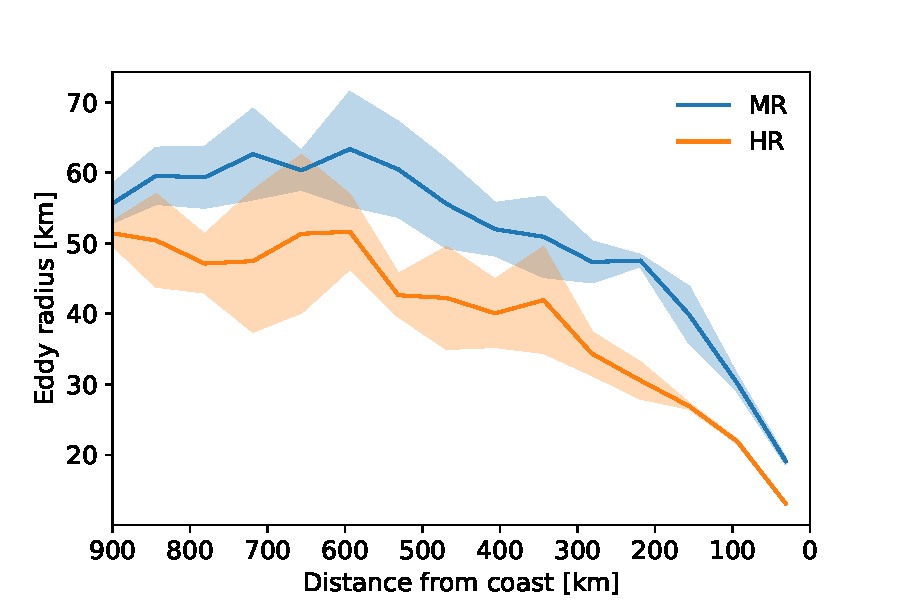
\includegraphics[width=8cm]{figures/result_eddies_d2c.pdf}
    \caption[Relative change of eddy radius with distance from coast]{\textbf{Eddy radius with distance from coast}.}
    \label{fig:meso_d2c}
\end{figure}

\begin{figure}
    \centering
    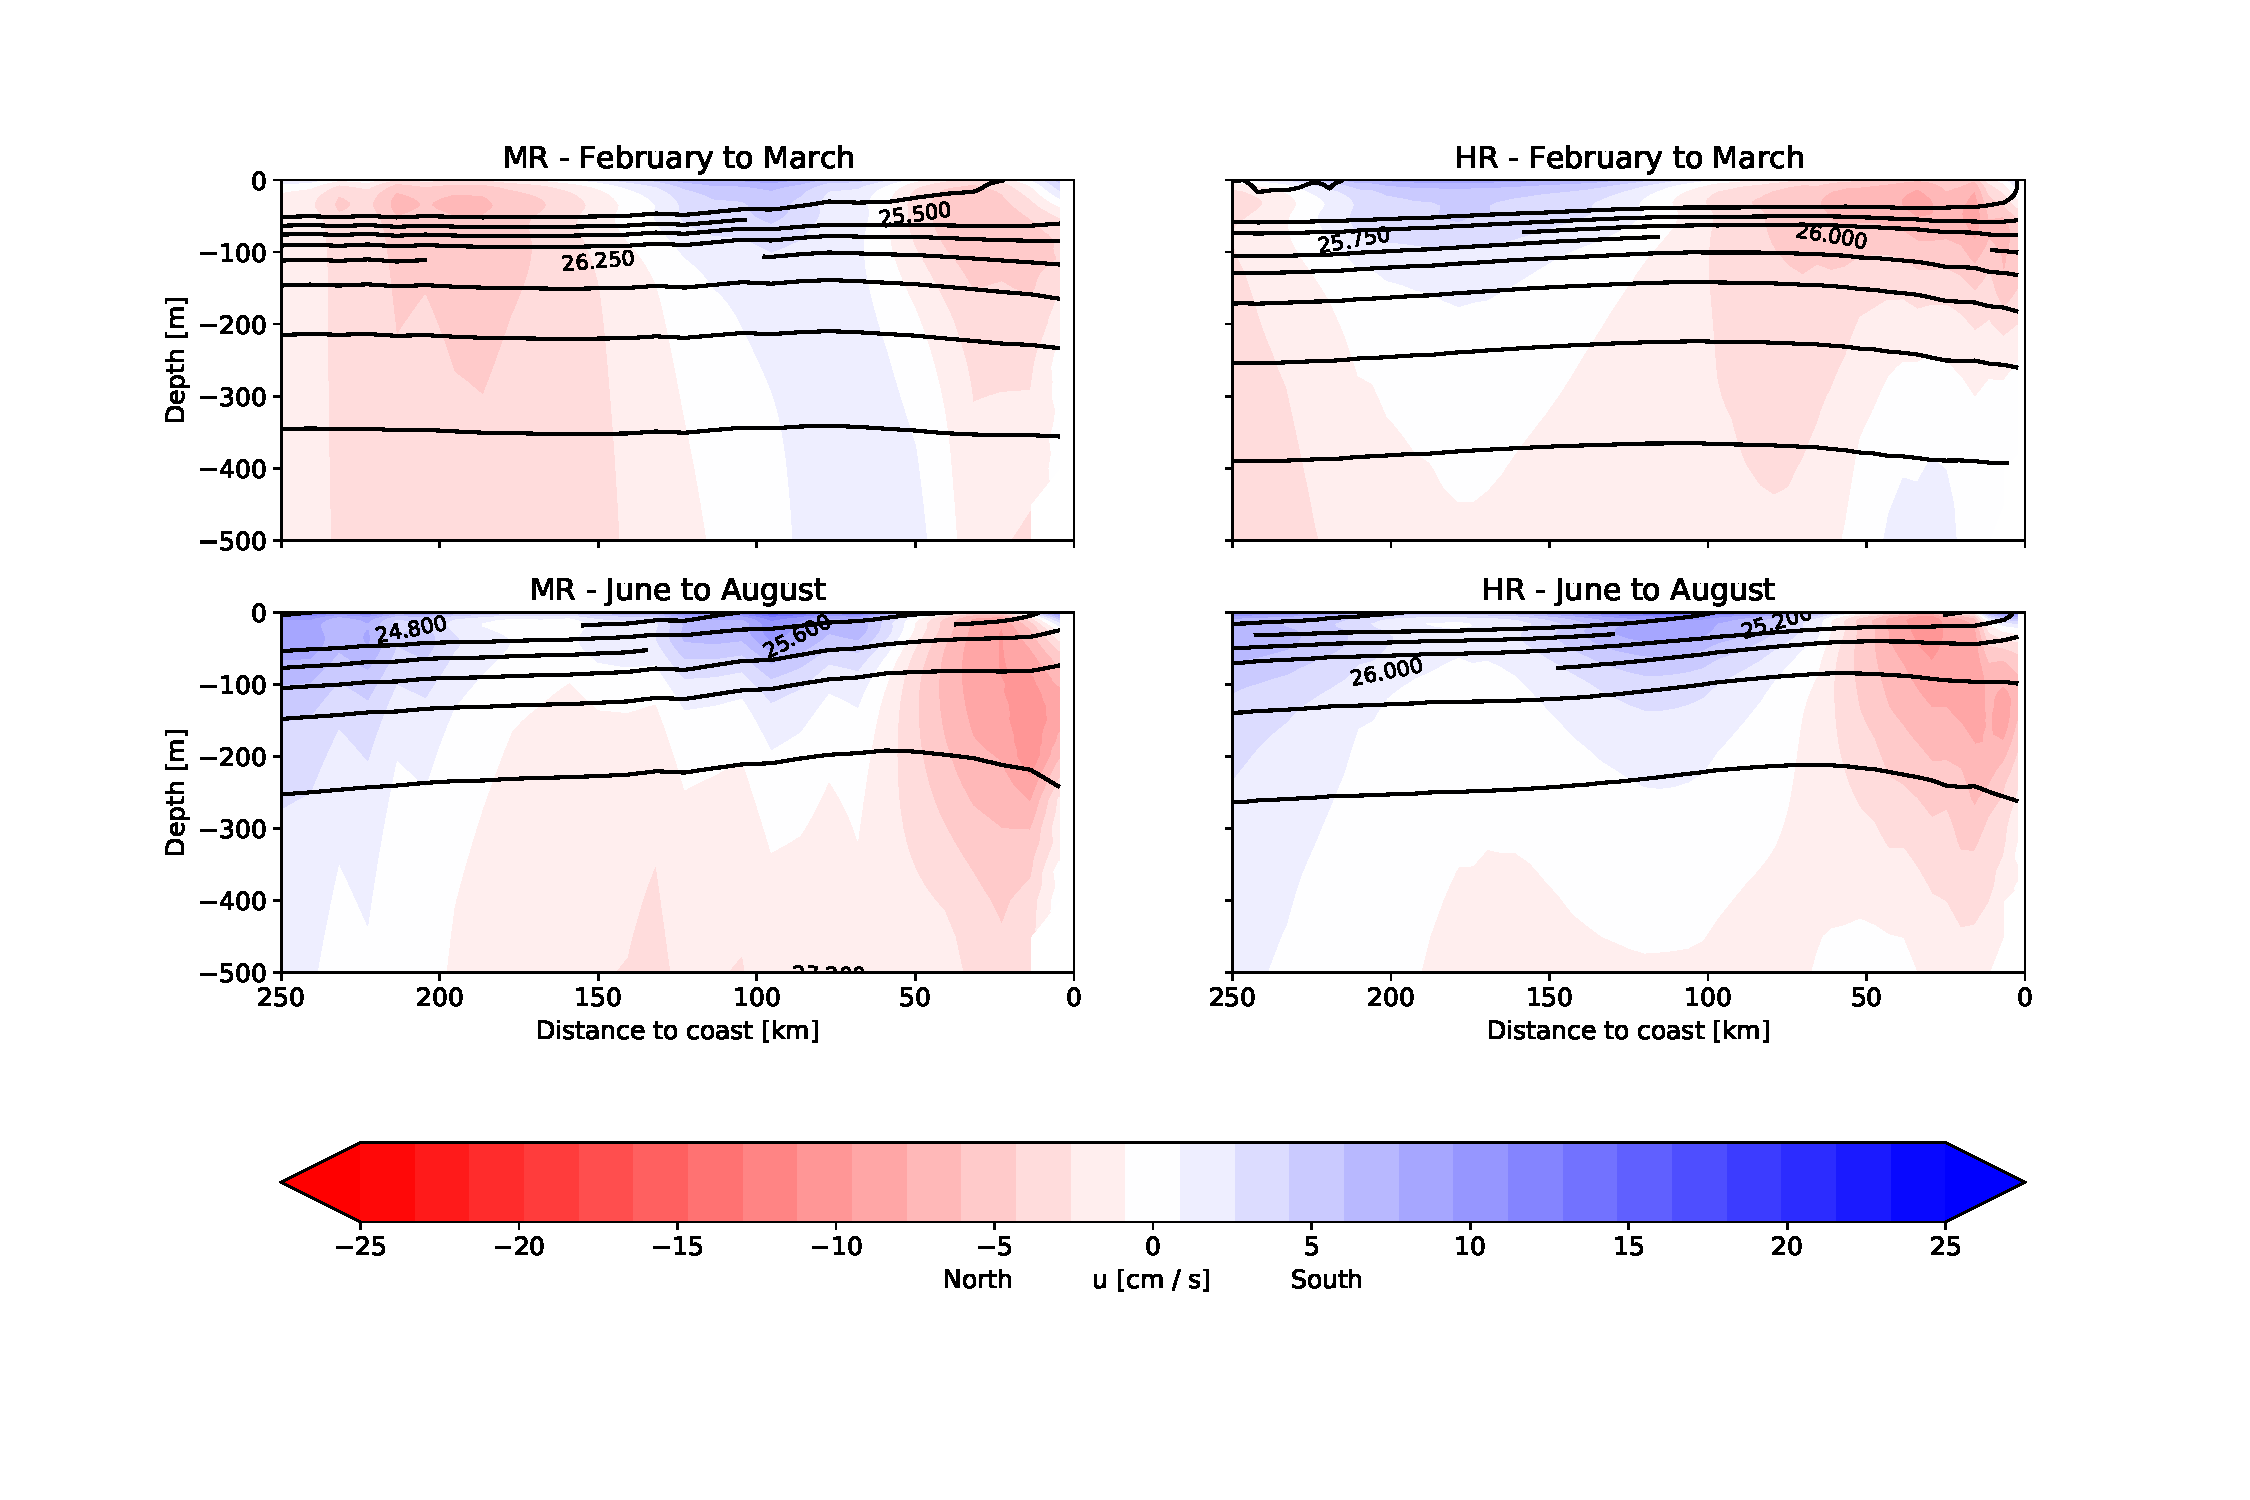
\includegraphics[width=16cm, trim=2cm 0 0 0]{figures/result_undercurrent.pdf}
    \caption[California Current and Undercurrent strength]{\textbf{California Current and Undercurrent strength}. The horizontal velocity component $u$ (parallel to coast) is shown for winter (top) and summer (bottom). The results for \ac{mr} are shown left and for \ac{hr} right. Contours represent isopycnals.}\label{fig:undercurrent}
\end{figure}

\begin{figure}
    \centering
    \hspace*{-0.2cm}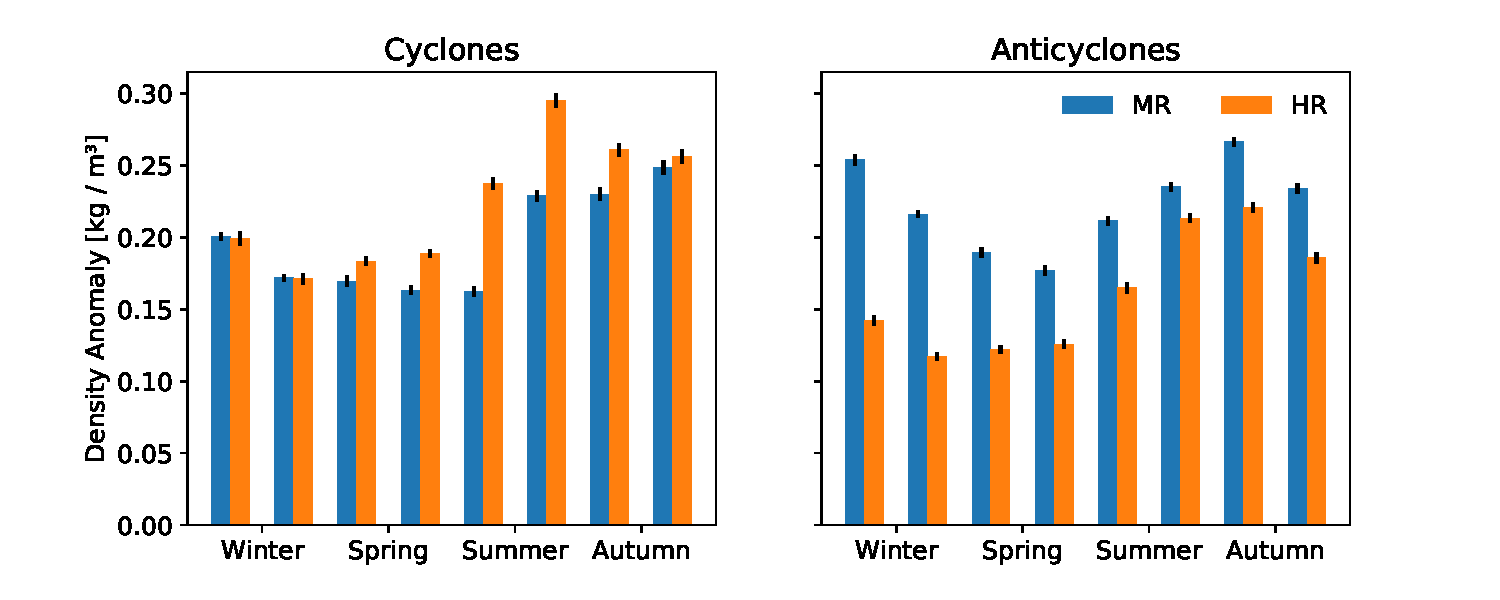
\includegraphics[width=16cm, trim=0 0 0 0]{../figures/result_eddies_density2}
    \caption[Offshore density anomaly (increased depth range)]{\textbf{Offshore density anomaly (increased depth range)}. Same as \autoref{fig:density-anomaly}, but averaged from 25m to 200m depth.}\label{fig:density-anomaly2}
\end{figure}

\begin{figure}
    \centering
    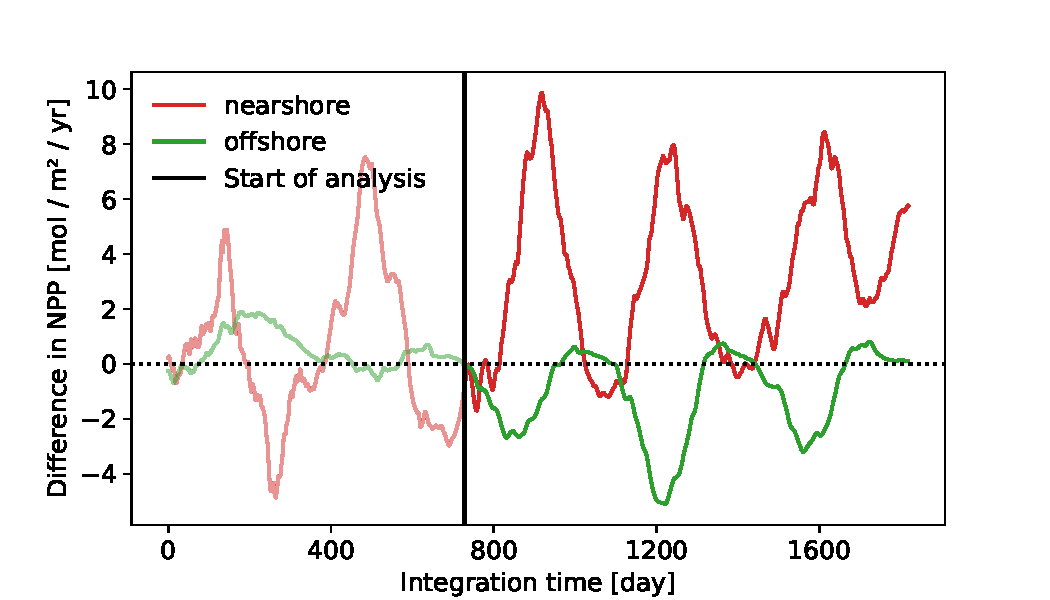
\includegraphics[width=10cm]{../figures/result_npp_drift.pdf}
    \caption[Temporal evolution of NPP difference]{\textbf{Temporal evolution of NPP difference} The difference MR - HR is shown for nearshore region (red) and offshore region (green). The curves were smoothed with a 120d rolling average. The solid black line denotes the start of analysis.}
    \label{fig:npp_drift}
\end{figure}